\documentclass[a4paper,12pt]{article} % тип документа

%  Русский язык
\usepackage[T2A]{fontenc}			% кодировка
\usepackage[utf8]{inputenc}			% кодировка исходного текста
\usepackage[english,russian]{babel}	% локализация и переносы

\usepackage{graphicx, scalerel}               % импорт изображений
\usepackage{wrapfig}                % обтекаемые изображения
\graphicspath{{pictures/}}          % обращение к подкаталогу с изображениями
\usepackage[14pt]{extsizes}         % для того чтобы задать нестандартный 14-ый размер шрифта
\usepackage[warn]{mathtext}         % русский язык в формулах
\usepackage{indentfirst}            % indent first
\usepackage[margin = 25mm]{geometry}% отступы полей
\usepackage[table,xcdraw]{xcolor}   % таблицы
\usepackage{amsmath,amsfonts,amssymb,amsthm,mathtools} % Математика
\usepackage{wasysym}                % ???
\usepackage{upgreek}                % ???  
\usepackage{caption}
\usepackage{multirow}
\captionsetup{labelsep=period}
\usepackage[font=small,labelfont=bf]{caption}
\usepackage{gensymb} % degree symbol
\usepackage{tikz}
\usetikzlibrary{positioning}


\begin{document}
	
	
	\begin{center}
		
		\textbf{НАЦИОНАЛЬНЫЙ ИССЛЕДОВАТЕЛЬСКИЙ УНИВЕРСИТЕТ \\ <<МОСКОВСКИЙ ФИЗИКО-ТЕХНИЧЕСКИЙ ИНСТИТУТ>>}
		\vspace{13ex}
		
		\textbf{Лабораторная работа 5.5.5\\ <<$\gamma$-спектроскопия>>}
		\vspace{40ex}
		
		\normalsize{Шумаков Иван Игоревич \\ студент группы Б01-009\\ 3 курс ФРКТ\\}
	\end{center}
	
	\vfill 
	
	\begin{center}
		г. Долгопрудный\\ 
		2022 г.
	\end{center}
	
	
	\thispagestyle{empty} % выключаем отображение номера для этой страницы
	\newpage

	\textbf{Цель работы:} Определение энергии и интенсивности дискретных гамма-линий от различных гамма-источников и их идентификация.\par
  \textbf{В работе используются:} Различные материалы, детектор.\par

	\section{Теоретические сведения}
		Основная задача спектрометрических измерений заключается в определении энергии, интенсивности дискретных гамма-линий от различных гамма-источников и их идентификации.
		Основными процессами взаимодействия гамма-излучения с веществом являются фотоэффект, эффект Комптона и образование электрон-позитронных пар. 
		Каждый из этих процессов вносит свой вклад в образование наблюдаемого спектра. Образующиеся при этих процессах электроны испытывают большое количество неупругих соударений с молекулами и атомами среды. 
		Неупругие соударения могут сопровождаться как ионизацией, так и возбуждением молекул или атомов среды. 
		В промежуточных же стадиях (при переходах возбужденных молекул или атомов в основное состояние, при рекомбинации электрических зарядов и т.п.) в веществе возникают кванты света различных длин волн, присущих данному веществу.
		При \textbf{фотоэффекте} кинетическая энергия электрона $ T_e = E_\gamma - I_i $, где $ I_i $ --- энергия ионизации $ i $-той оболочки атома. 
		Фотоэффект особенно существенен для тяжелых веществ, где он идет с заметной вероятностью даже при высоких энергиях гамма-квантов. \
		В легких веществах фотоэффект становится заметен лишь при относительно небольших энергиях гамма-квантов. 
		Наряду с фотоэффектом, при котором вся энергия гамма-кванта передается атомному электрону, взаимодействие гамма-излучения со средой может приводить к его рассеянию, т.е. отклонению от первоначального направления распространения на некоторый угол.
		При \textbf{эффекте Компотна} происходит упругое рассеяние фотона на свободном электроне, сопровождающееся изменением длины волны фотона (реально этот процесс происходит на слабо связанных с атомом внешних электронах). 
		Максимальная энергия образующихся комптоновских электронов соответствует рассеянию гамма-квантов на $ 2\pi $ и равна
		\begin{equation}\label{E_compton}
			E_{c_max} = \dfrac{\hbar \omega}{1 + \dfrac{m_ec^2}{2\hbar\omega}}
		\end{equation}
		При достаточно высокой энергии гамма-кванта наряду с фотоэффектом и эффектом Комптона может происходить третий вид взаимодействия гамма-квантов с веществом – \textbf{образование электрон-позитронных пар}. 
		При этом если процесс образования пары идет в кулоновском поле ядра или протона, то энергия образующегося ядра отдачи оказывается весьма малой, так что пороговая энергия гамма-кванта, необходимая для образования пары, практически совпадает с удвоенной энергией покоя электрона $ E_0 = 2m_ec^2 =1,022  $МэВ.
		Появившийся в результате процесса образования пар электрон теряет свою энергию на ионизацию среды. Таким образом, вся энергия электрона остается в детекторе. Позитрон будет двигаться до тех пор, пока практически не остановится, а затем аннигилирует с электроном среды, в результате чего появятся два гамма-кванта. Т.е., кинетическая энергия позитрона также останется в детекторе. Далее возможны три варианта развития событий:	
		а) оба родившихся гамма-кванта не вылетают из детектора, и тогда вся энергия первичного гамма-кванта останется в детекторе, а в спектре появится пик с $ E = E_\gamma $;
		б) один из родившихся гамма-квантов покидает детектор, и в спектре появляется пик, соответствующий энергии $  E = E_\gamma - E0 $, где $ E_0 = m_ec^2 = $ 511 кэВ;
		в) оба родившихся гамма-кванта покидают детектор, и в спектре появля- ется пик, соответствующий энергии $  E = E_\gamma - 2E0 $, где $ 2E_0 = 2m_ec^2 = $ 1022 кэВ;
		Таким образом, любой спектр, получаемый с помощью гамма-спектрометра, описывается несколькими компонентами, каждая из которых связана с определенным физическим процессом. 
		Как описано выше, основными физическими процессами взаимодействия гамма-квантов с веществом являются фотоэффект, эффект Комптона и образование электрон-позитронных пар, и каждый из них вносит свой вклад в образование спектра. 
		Помимо этих процессов, добавляются экспонента, связанная с наличием фона, пик характеристического излучения, возникающий при взаимодействии гамма-квантов с окружающим веществом, а также пик обратного рассеяния, образующийся при энергии квантов $ Е_\gamma \gg mc^22/2 $ в результате рассеяния гамма-квантов на большие углы на материалах конструктивных элементов детектора и защиты. 
		Положение пика обратного рассеяния определяется по формуле ($ E $ --- энергия фотопика):
		\begin{equation}\label{Eobr}
			E_{\text{обр}} = \dfrac{E}{1 + \dfrac{2E}{mc^2}}
		\end{equation}
		Энергетическим разрешением спектрометра называется величина
		\begin{equation}\label{Ri = dE/E}
			R_i = \dfrac{\Delta E_i}{E_i}
		\end{equation}
		т.е. отношение ширины пика полного поглощения (измеренной на полувысоте) к регистрируемой энергии пика поглощения. Это значение $ E_i \propto \overline{n_i} $ --- числу частиц на выходе ФЭУ. 
		При этом  $ \Delta E_i \propto \overline{\Delta n_i} = \sqrt{\overline{n_i}} $ --- ширина пика пропорциональна среднеквадратичной флуктуации, которая равна корню из числа частиц. 
		Таким образом, наша формула \eqref{Ri = dE/E} примет вид
		\begin{equation}\label{Ri = c/E}
			R_i = \dfrac{\mathrm{const}}{\sqrt{E_i}}
		\end{equation}

	\section{Ход работы}
		В ходе работы были получены спектры материалов:
		\begin{figure}[h!]
      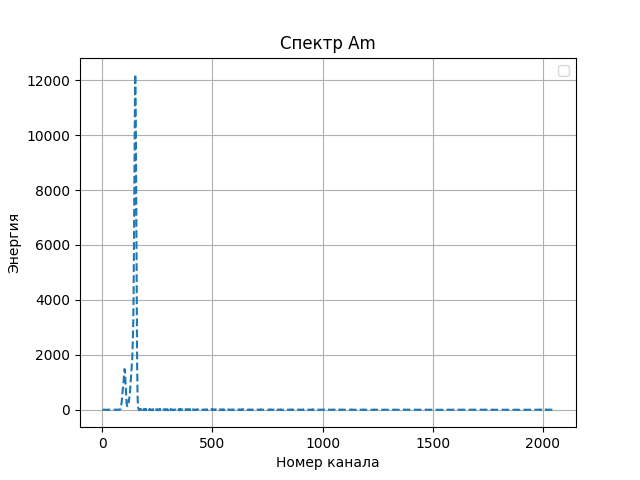
\includegraphics[width=0.55\textwidth]{img/Am.png}
      \centering
      \caption{Спектр Am}
    \end{figure}\par
		\begin{figure}[h!]
      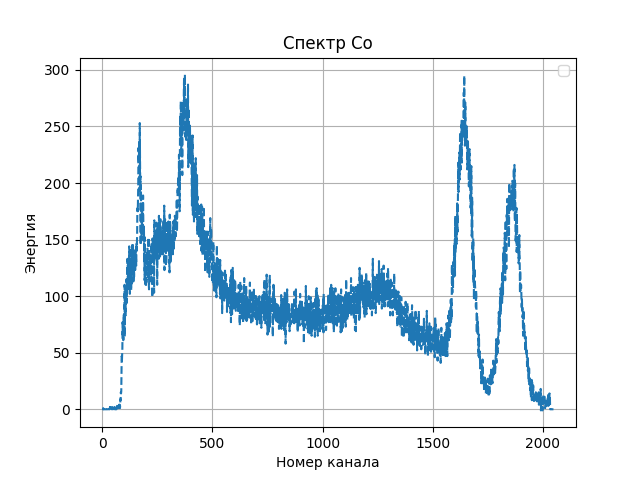
\includegraphics[width=0.55\textwidth]{img/Co.png}
      \centering
      \caption{Спектр Co}
    \end{figure}\par
		\begin{figure}[h!]
      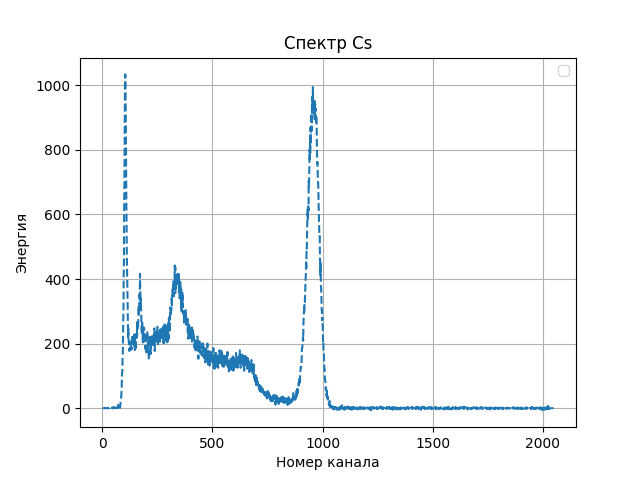
\includegraphics[width=0.55\textwidth]{img/Cs.png}
      \centering
      \caption{Спектр Cs}
    \end{figure}\par
		\begin{figure}[h!]
      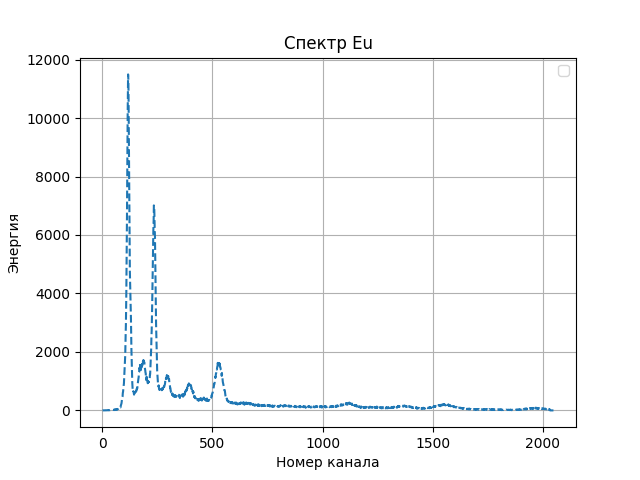
\includegraphics[width=0.55\textwidth]{img/Eu.png}
      \centering
      \caption{Спектр Eu}
    \end{figure}\par
		\begin{figure}[h!]
      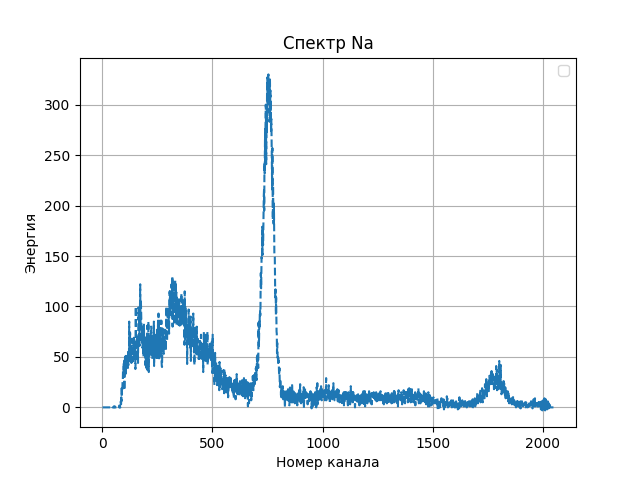
\includegraphics[width=0.55\textwidth]{img/Na.png}
      \centering
      \caption{Спектр Na}
    \end{figure}\par
	\newpage
		\subsection*{Am}
			При $\alpha$-распаде америция происходит испускание мягких $\gamma$-квантов:
			\begin{figure}[h!]
				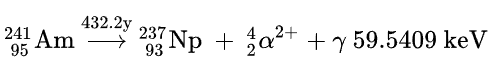
\includegraphics[width=0.7\textwidth]{img/Am-alpha.png}
				\centering
				\caption{Распад америция}
			\end{figure}\par
			Таким образом пику на 94 канале соответствует квант 59 кэВ.
		
		\subsection*{Co}
			Для кобальта характерны фотопики на энергиях 1.33 мэВ и 1.17 мэВ.
			Им соответствуют каналы 1856 и 1638.
			\begin{figure}[h!]
				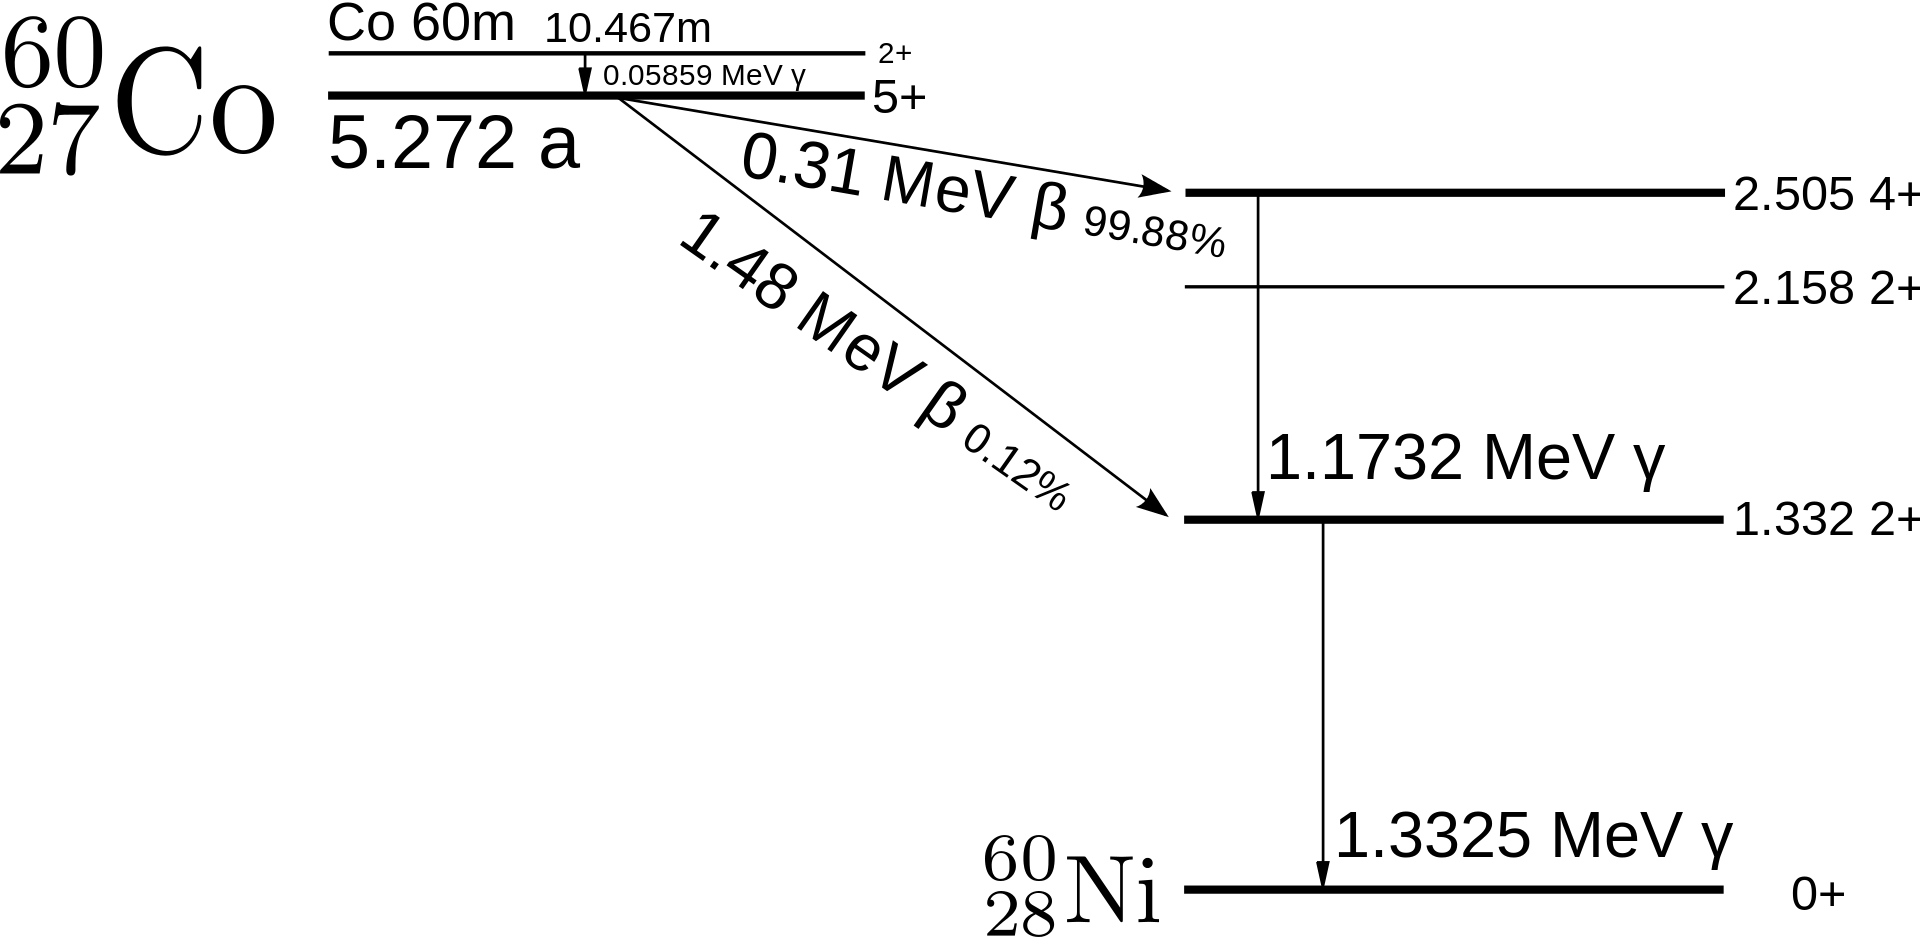
\includegraphics[width=0.65\textwidth]{img/Cobalt-60m-decay.png}
				\centering
				\caption{Уровни кобальта}
			\end{figure}\par
	\newpage
		\subsection*{Cs}
			Фотопик цезия имеет энергию 0.66 мэВ. 
			Ему соответствует 953 канал.
			\begin{figure}[h!]
				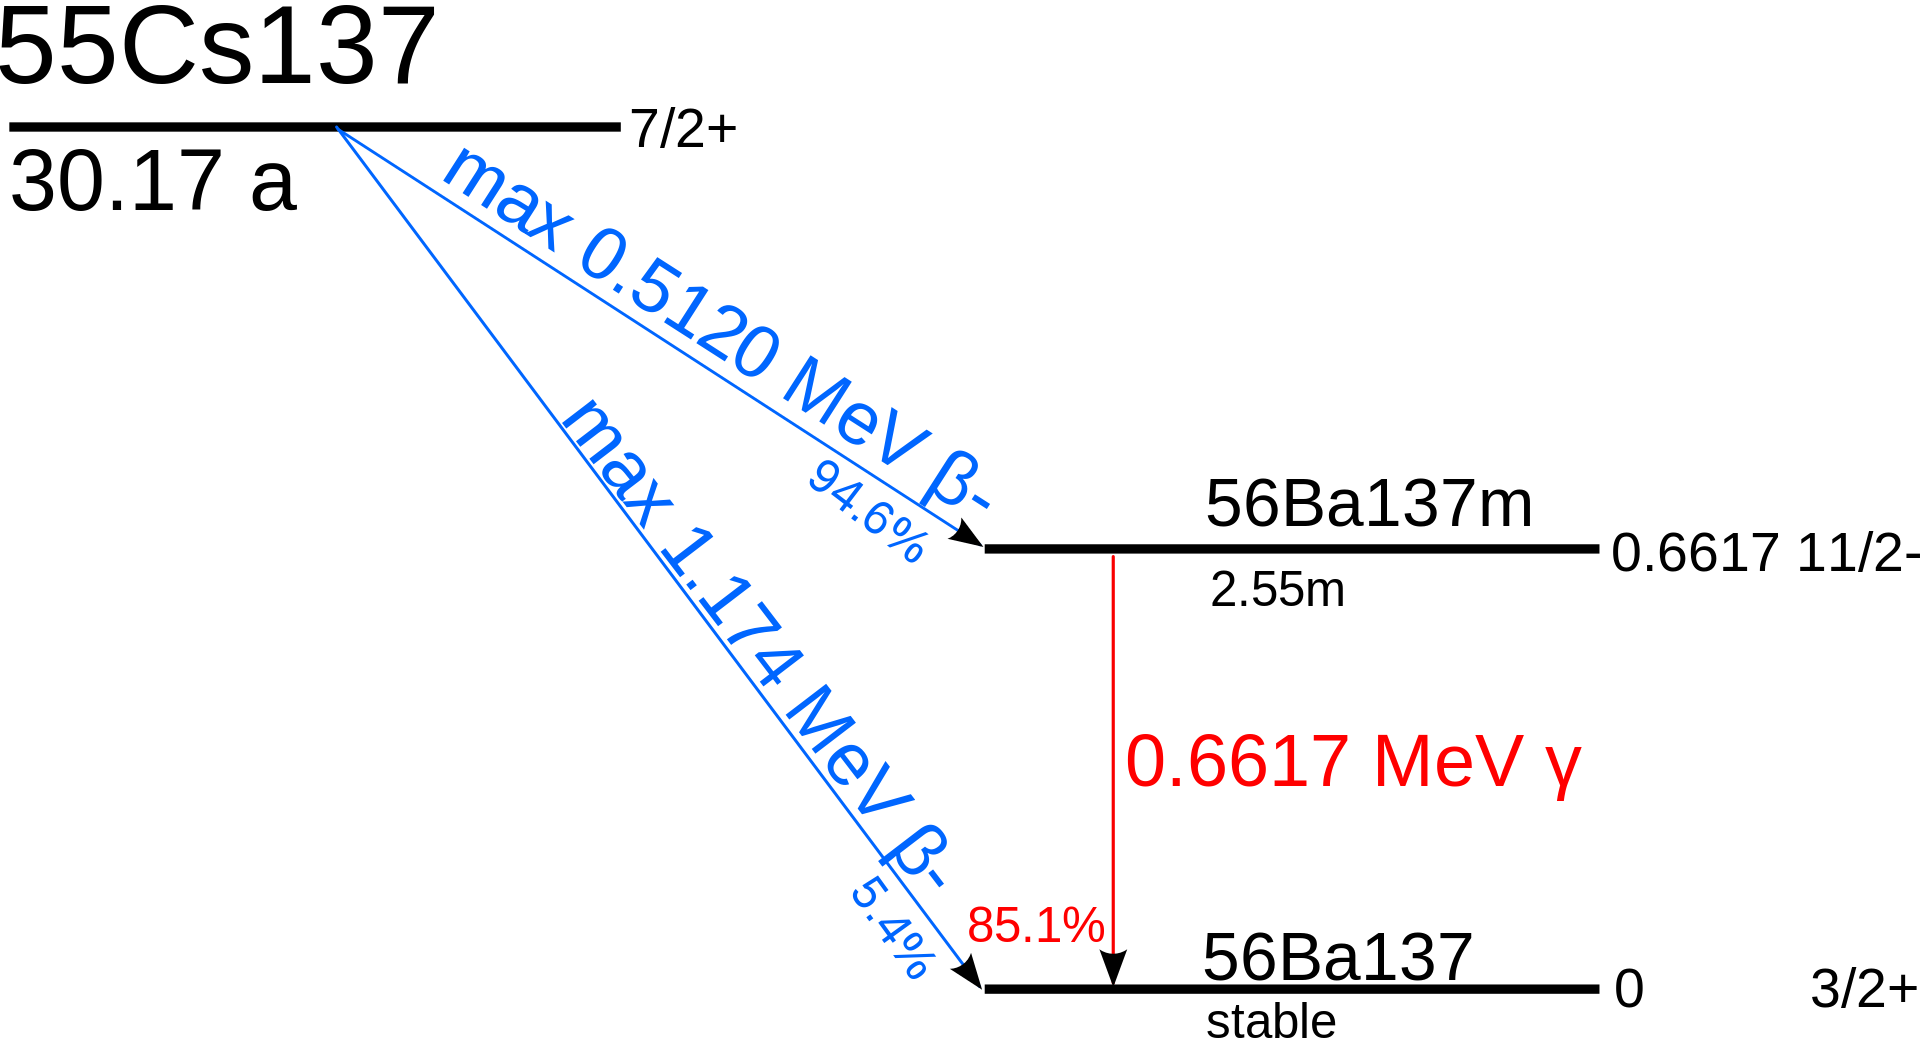
\includegraphics[width=0.65\textwidth]{img/Cs-137-decay.png}
				\centering
				\caption{Уровни цезия}
			\end{figure}\par
		
		\subsection*{Eu}
			У европия наблюдается много фото-пиков.
			Таблица, со всеми линиями спектра европия:
			\begin{figure}[h!]
				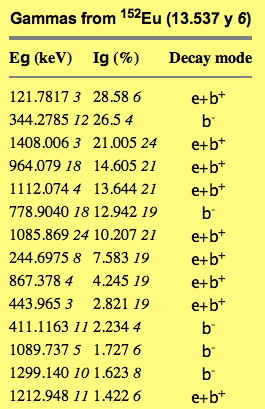
\includegraphics[width=0.4\textwidth]{img/152Eu.jpg}
				\centering
				\caption{Спектр цезия}
			\end{figure}\par
			Соответствия каналов и фото-пиков:
			\begin{itemize}
				\item 1965 канал - 1.41 мэВ
				\item 1550 канал - 1.09 мэВ
				\item 1362 канал - 0.96 мэВ
				\item 1112 канал - 0.78 мэВ
			\end{itemize}
		
		\subsection*{Na}
			Фотопик натрия соответствует энергии 1.27 мэВ.
			В эксперименте это был 1779 канал.
			\begin{figure}[h!]
				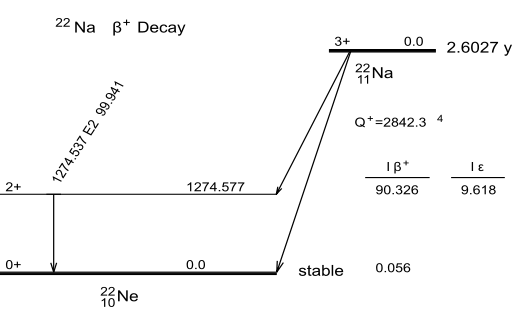
\includegraphics[width=0.7\textwidth]{img/Na-22-decay.png}
				\centering
				\caption{Спектр натрия}
			\end{figure}\par
	\newpage
		\subsection*{Анализ данных}
		Фотопики каждого из элементов:
		\begin{table}[h]
			\centering
			\begin{tabular}{|c|c|c|}
			\hline
			Элемент & Энергия [кэВ]		  & Канал \\ \hline
			Am      & 59                & 94    \\ \hline
			Co      & 1330              & 1856  \\ \hline
			Co      & 1170              & 1638  \\ \hline
			Cs      & 660               & 953   \\ \hline
			Eu      & 1410              & 1965  \\ \hline
			Eu      & 1090              & 1550  \\ \hline
			Eu      & 960               & 1362  \\ \hline
			Eu      & 780               & 1112  \\ \hline
			Na      & 1270              & 1779  \\ \hline
			\end{tabular}
		\end{table}\par
		По полученным данным была построена зависимость энергии от номера канала
		\begin{figure}[h!]
      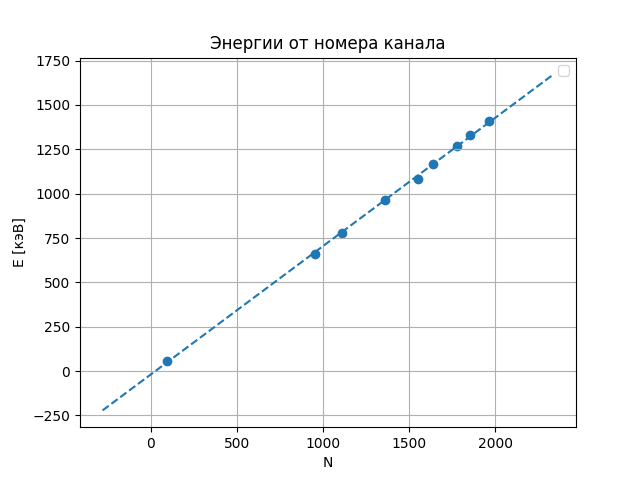
\includegraphics[width=0.7\textwidth]{img/Chan-approx.png}
      \centering
      \caption{Перевод номера канала в энергию}
    \end{figure}\par
		Уравнение по данномк приближению:
		\begin{equation}
			E = 72.3 * 10^{-2} * N - 19.3
		\end{equation}
		Погрешность коэффициентов этого уравнения оценим как последнюю значущую цифру $\delta \approx 0.01$.\par
	\newpage
		\subsection*{Энергетическое разрешение}	
			С помощью этого уравнения была посчитана ширина пиков на полувысоте и энергетическое разрешение измерителя:
			\begin{table}[h]
				\centering
				\begin{tabular}{|c|c|c|c|}
				\hline
				Элемент & $E$  [ кэВ ]  & $\Delta E$ [кэВ]     & R     \\ \hline
				Am      & 59            & 8.6                   & 0.150 \\ \hline
				Co      & 1330          & 65                    & 0.048 \\ \hline
				Co      & 1170          & 58                    & 0.049 \\ \hline
				Cs      & 660           & 43                    & 0.065 \\ \hline
				Eu      & 1410          & -                     & -     \\ \hline
				Eu      & 1090          & -                     & -     \\ \hline
				Eu      & 960           & -                     & -     \\ \hline
				Eu      & 780           & -                     & -     \\ \hline
				Na      & 1270          & 54                    & 0.043 \\ \hline
				\end{tabular}
			\end{table}\par
			По этим данным был построен график зависимости $R^2 f(1 / E)$:
			\begin{figure}[h!]
				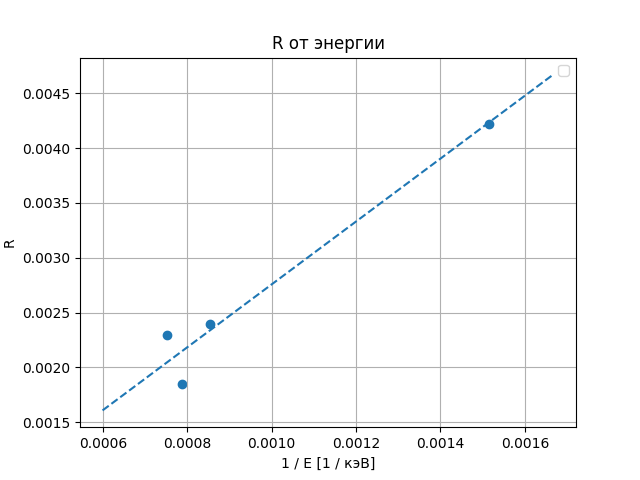
\includegraphics[width=0.7\textwidth]{img/R.png}
				\centering
				\caption{Энергетическое разрешение}
			\end{figure}\par
			Линейное приближение хорошо отображает зависимость и график проходит через ноль.
			Таким образом можно сделать вывод, что энергетическое разрешение зависит от энергии как:
			\begin{equation}
				R = \frac{const}{\sqrt{E}}
			\end{equation}
	\newpage
		\subsection*{Пик обратного рассеяния}
			В результате фотоэффекта излучение происходит во все стороны, поэтому рядом с фотопиком присутствует пик обратного рассеяния, обусловеленный отражением излучения от среды.
			Фотопики также присутствуют и на маленьких энергиях.
			Рядом с ними пики обратного рассеяния видны четче, поскольку в этой области энергетическое разреешение детектора выше.\par
			Пики обратного рассеяния и соответствующие им фотопики:
			\begin{table}[h!]
				\centering
				\begin{tabular}{|c|c|c|}
				\hline
				Элемент & $E_\text{фото}$ [кэВ] & $E_{\text{обр}}$ [кэВ] \\ \hline
				Am      & 61                         & 27                         \\ \hline
				Co      & 1329                       & 240                        \\ \hline
				Cs      & 660                        & 195                        \\ \hline
				Eu      & 124                        & 87                         \\ \hline
				Na      & 511                        & 184                        \\ \hline
				\end{tabular}
			\end{table}\par
			График зависимти энергии пика обратьного рассеяния от энергии фотопика:
			\begin{figure}[h!]
				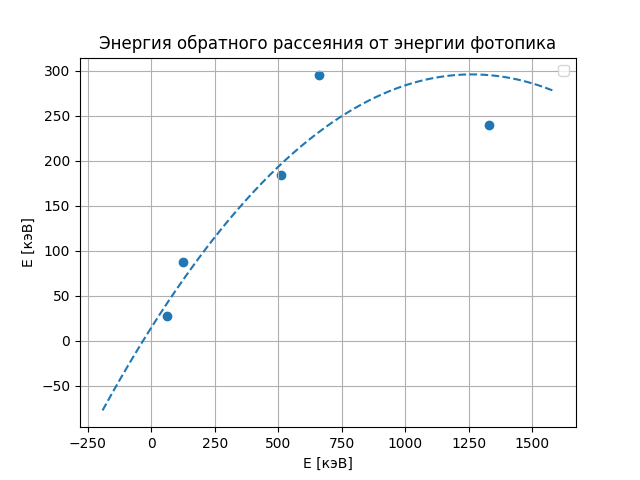
\includegraphics[width=0.7\textwidth]{img/Back.png}
				\centering
				\caption{Обратное рассеяние}
			\end{figure}\par
			Данная зависимоть примерно соответствует теоретической:
			\begin{equation}
				E_{\text{обр}} = \frac{E}{1 + 2 E / mc^2}
			\end{equation}
	\section{Вывод}
		
\end{document}